\documentclass{article}
\usepackage[utf8]{inputenc}
\usepackage{amsmath} % Para un mejor formato de ecuaciones
\usepackage{amssymb} % Para símbolos matemáticos
\usepackage{tikz}    % Para la representación geométrica

\title{Raíces Sextas de la Unidad}
\author{Mauricio Odreman Vera}
\date{}

\begin{document}
	
	\maketitle
	
	\section*{(a) Encuentre las seis raíces sextas de 1}
	
	Para resolver la ecuación $z^6 = 1$, expresamos el número $1$ en su forma polar general:
	\[ 1 = \cos(2k\pi) + i\sin(2k\pi) \]
	
	Aplicando la fórmula de De Moivre para las raíces complejas, obtenemos:
	\[ z_k = \cos\left(\frac{2k\pi}{6}\right) + i\sin\left(\frac{2k\pi}{6}\right) = \cos\left(\frac{k\pi}{3}\right) + i\sin\left(\frac{k\pi}{3}\right) \]
	
	Donde $k = 0, 1, 2, 3, 4, 5$. Evaluando para cada valor de $k$, obtenemos las seis raíces en forma binómica:
	
	\begin{align*}
		z_0 &= \cos(0) + i\sin(0) = 1 \\
		z_1 &= \cos\left(\frac{\pi}{3}\right) + i\sin\left(\frac{\pi}{3}\right) = \frac{1}{2} + \frac{\sqrt{3}}{2}i \\
		z_2 &= \cos\left(\frac{2\pi}{3}\right) + i\sin\left(\frac{2\pi}{3}\right) = -\frac{1}{2} + \frac{\sqrt{3}}{2}i \\
		z_3 &= \cos(\pi) + i\sin(\pi) = -1 \\
		z_4 &= \cos\left(\frac{4\pi}{3}\right) + i\sin\left(\frac{4\pi}{3}\right) = -\frac{1}{2} - \frac{\sqrt{3}}{2}i \\
		z_5 &= \cos\left(\frac{5\pi}{3}\right) + i\sin\left(\frac{5\pi}{3}\right) = \frac{1}{2} - \frac{\sqrt{3}}{2}i
	\end{align*}
	
	\section*{(b) Represente las raíces geométricamente}
	
	En el plano complejo, las raíces se distribuyen uniformemente sobre la circunferencia unitaria ($|z| = 1$), formando los vértices de un hexágono regular inscrito.
	
	\begin{center}
		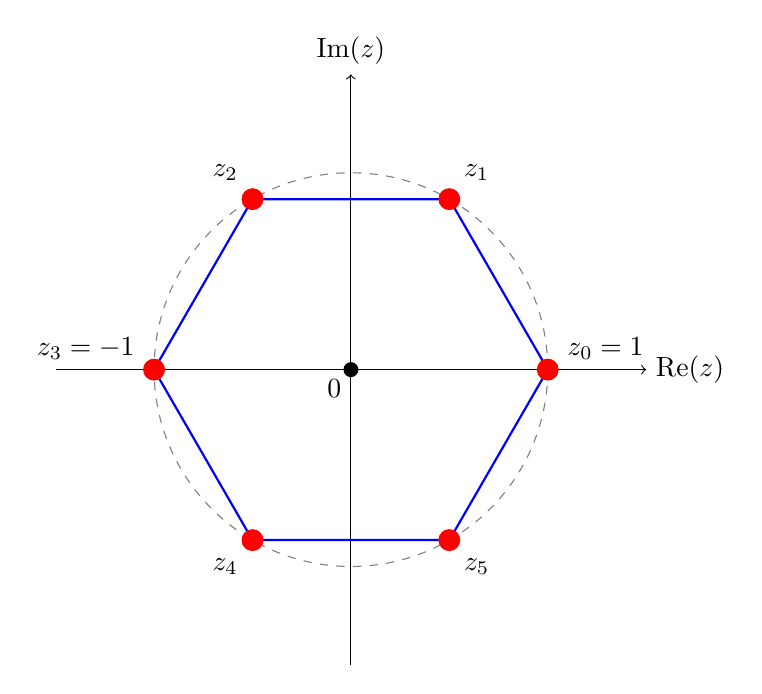
\begin{tikzpicture}[scale=2.5]
			% Ejes coordenados
			\draw[->] (-1.5,0) -- (1.5,0) node[right] {$\text{Re}(z)$};
			\draw[->] (0,-1.5) -- (0,1.5) node[above] {$\text{Im}(z)$};
			
			% Circunferencia unitaria
			\draw[dashed, gray] (0,0) circle (1);
			
			% Dibujar el hexágono
			\draw[blue, thick] (0:1) -- (60:1) -- (120:1) -- (180:1) -- (240:1) -- (300:1) -- cycle;
			
			% Puntos de las raíces y etiquetas
			\foreach \angle/\label/\pos in {
				0/{z_0=1}/above right,
				60/{z_1}/above right,
				120/{z_2}/above left,
				180/{z_3=-1}/above left,
				240/{z_4}/below left,
				300/{z_5}/below right} {
				\filldraw[red] (\angle:1) circle (1.5pt);
				\node[\pos] at (\angle:1.05) {$\label$};
			}
			
			% Origen
			\filldraw (0,0) circle (1pt) node[below left] {$0$};
		\end{tikzpicture}
	\end{center}
	
\end{document}
